\begin{figure}
  \setlength{\unitlength}{\textwidth}
       
        \begin{picture}(1,0.52)

      % % % Parkinson Data 
      \put(0.025,0.27){\includegraphics[width=0.5\unitlength]{../FnP/gnuplot/velocity_amp_collapsed_parkinson.eps}}
      \put(0.495,0.27){\includegraphics[width=0.5\unitlength]{../FnP/gnuplot/velocity_amp_collapsed_re165.eps}}
      
      \put(0.025,0.02){\includegraphics[width=0.5\unitlength]{../FnP/gnuplot/mean_power_collapsed_parkinson.eps}}
      \put(0.495,0.02){\includegraphics[width=0.5\unitlength]{../FnP/gnuplot/mean_power_collapsed_re_165.eps}}
      
      
      \put(0.23,0.00){ $c\rho\mathcal{A}U$}
      \put(0.73,0.00){ $c\rho\mathcal{A}U$}
      
      \put(0.01,0.405){$\frac{V}{D}$}
      
      \put(0,0.13){$\frac{P_{m}}{\rho \mathcal{A}U^3 }$}
      \put(0.085,0.475){\small(a)}
      \put(0.555,0.475){\small(b)}
      \put(0.095,0.225){\small(c)}
      \put(0.555,0.225){\small(d)}
      
    \end{picture}

  \caption{ Velocity amplitude and mean power as a function of the damping factor. (a) and (c)  are calculated using input $C_y$ data at $Re=22300$ obtained by \cite{Parkinson1964} at three different damping ratios: $\zeta=0.0125$ (\ding{83}), $\zeta=0.015$ (\ding{116}) and $\zeta=0.0175$ (\ding{108}). (b)and (d)  are at $Re=165$ are calculated from the fixed body simulations at three different damping ratios: $\zeta=0.075$ ($\times$), $\zeta=0.1$ (\ding{117}) and $\zeta=0.15$ (+). The collapsed data implies that there is no frequency selection and the tuning parameter of the mechanical side of the system is the damping constant to obtain an optimum power output.}
    \label{fig:collpased_data}
\end{figure}

\ %vspace{10cm}
